\documentclass{article}
\author{Anjal Doshi, Nasser Al-Ghamdi, Nick Rohde}
\title{CSS 534 Program 5 Report}
\date{11$^{th}$ of December 2018}

\usepackage[margin=1in]{geometry} % page margins
\usepackage{graphicx} % images
\graphicspath{ {./images/} } % image path
\usepackage{xcolor} % link colours
\usepackage{hyperref} % links
\usepackage{listings} % code
\usepackage{color} % syntax colours
\usepackage{caption} % figure captions

\definecolor{dkgreen}{rgb}{0,0.6,0}
\definecolor{gray}{rgb}{0.5,0.5,0.5}
\definecolor{mauve}{rgb}{0.58,0,0.82}

\lstset{frame=tb,
	language=Java,
	aboveskip=3mm,
	belowskip=3mm,
	showstringspaces=false,
	columns=flexible,
	basicstyle={\small\ttfamily},
	numbers=none,
	numberstyle=\tiny\color{gray},
	keywordstyle=\color{blue},
	commentstyle=\color{dkgreen},
	stringstyle=\color{mauve},
	breaklines=true,
	breakatwhitespace=true,
	tabsize=2
}

\hypersetup
{
	colorlinks=true,
	citecolor=black,
	filecolor=black,
	linkcolor=black,
	urlcolor=blue,
	linktoc=all,
	linkcolor=blue,
}

\begin{document}
\maketitle
\tableofcontents
\pagebreak
	
	\section{Overview} \label{OVERVIEW}
		Our program five was a parallel implementation of the Simulated Annealing (SA) algorithm. The SA algorithm is a local search based algorithm which uses thermodynamic functions to simulate a system going from a heated state to a cooled state, similar to metal being annealed. The algorithm uses two main loops as part of this simulation. \\
		
		The first of these loops (we will refer to this as the outer loop) simulates the cooling of the system, the initial heat of the system is set to an arbitrary value (in our case 100) and cools until it reaches another arbitrary threshold (in our case 0.001). In this loop we modify the temperature according to equation \hyperref[E_TEMP]{Equation 1} at the conclusion of each iteration. \\
		
		The second loop (we will refer to this as the inner loop) is independent of the heat and is the optimization step, in this loop, we allow the system to stabilize by running a local search for an arbitrary number of iterations (in our case 1,000,000); in this loop, we find a new neighboring solution to our current candidate solution at each step. If a new solution is better than our previous solution, we will always accept it and move our search to its neighborhood; if it is worse, we will calculate an acceptance probability, $p$, using equation \hyperref[E_AP]{Equation 2} and generate a uniformly distributed random number, $r$, if $p > r$ we accept our new (worse) solution, otherwise we reject it. \\
		
		Throughout the process, we keep track of our overall best solution and update it as needed, once the process finishes, this solution is returned as the result.\\
		
		\begin{equation}\label{E_TEMP}
			T(k) = \frac{T(k-1)}{log(k)} \qquad k = annealing~step
		\end{equation}

		\begin{equation}\label{E_AP}
			p(S_i) = e^{-\frac{(-S_{i} + S_{i-1} )}{T}} \qquad S_i = i^{th}~solution; \quad T = current~heat
		\end{equation}
	
	\section{Documentation} \label{DOCUMENTATION}
		\subsection{MPI Java} \label{D_MPI}
			Our MPI Java implementation spread out computation over multiple MPI nodes by running SA on each node individually. \hyperref[F1]{Figure 1} shows a flow diagram of our design. \\
			
			Each node received a different random seed, to ensure they did not follow the same path, and a different starting point. At the conclusion of each outer-loop iteration, all MPI nodes exchanged their current best solution, and all nodes then adopted the best solution in the cluster. This was done to prevent having nodes follow a dead-end path and keep all nodes searching an area of the search space known to contain good solutions. This can also lead to premature convergence, however, this was the only feasible option we could think of that did not destroy the performance by introducing an immense amount of communication. \\
			
			Another change that was made to the sequential version is that we divided the number of inner loop iterations over the nodes, i.e. if we ran SA for 100 inner loop iterations over 4 nodes, each node would only run 25 iterations. This approach is feasible as long as the number of inner loop iterations is sufficiently large.
		
			\begin{figure}\label{F1}
				\caption{Program Flow of the MPI Implementation.}
				\centering
				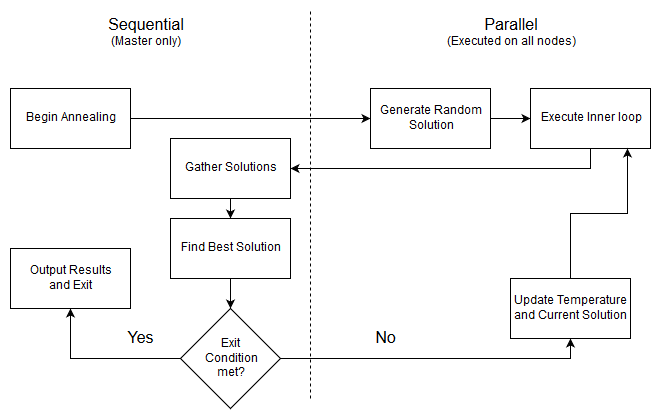
\includegraphics[scale=0.65]{mpi_flow.png}
			\end{figure}
		
		\subsection{MapReduce} \label{D_MR}
		    Our MapReduce implementation spread out computation over multiple nodes using multiple mappers where each mapper runs its own SA. \hyperref[F2]{Figure 2} shows a flow diagram of our design. \\
			
			Each mapper receives a line from the cities file. Each line consists of all the city coordinate pairs. The map function then generates a solution from the input file and sets it as the initial best solution. This initial Solution is used as the input to the SA algorithm. After generating their respective best solution, each mapper collects the output with the $\langle1, Best-Solution\rangle$ as the $\langle key, value\rangle$ pair. Each mapper assigns the same key to their solution so that only a single reducer is created. This is so that, the reducer collects the output from all the solution and then selects the solution with the best distance. The output of the reducer is the best solution from all the mappers and is then stored in the output directory.
			
			\begin{figure}\label{F2}
				\caption{Program Flow of the MapReduce Implementation.}
				\centering
				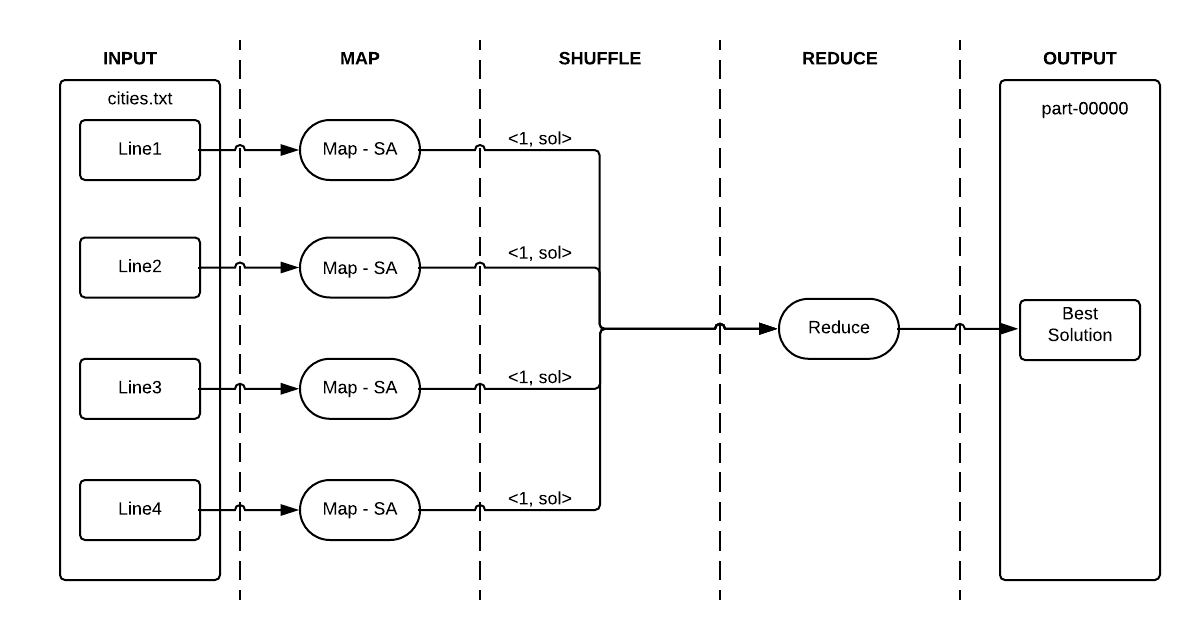
\includegraphics[scale=0.6]{mapreduce_flow.png}
			\end{figure}
		
		\subsection{Spark} \label{D_SPARK}
		The Spark version is acccepting additional input, number of partitions. The following steps illustrate execution process in Spark:
		\begin{enumerate}
		\item Generate initial solution randomly and broadcast.
		\item Generate a list of 12 (maximum number of executors at the server) random-generators each with a different seed and broadcast once. Each executor uses its id to retrieve its generator; thus, each one guaranteed to generate different solutions.
		\item Initialize RDD file:
		\begin{itemize} 
			\item Contain initial solution as many as the number of partitions.
			\item Partition the RDD into the given number of partitions, each partition contains only one initial solution.
		\end{itemize}
		\item Starting the outer loop same as the sequential algorithm:
		\begin{itemize} 
			\item The inner loop uses map transformation to produce the best solution same as in sequential but the number of iterations (user input) is divided by the number of partitions.
		    \item Apply reduce action to get the best solution among all partitions.
		    \item Broadcast the best solution.
		    \item Reduce the heat and repeat this step (\#4) until reaching the minimum heat.
		\end{itemize}
		\item Output the best solution.
		\end{enumerate}

		\begin{figure}\label{F1}
			\caption{Program Flow of the Spark Implementation.}
			\centering
			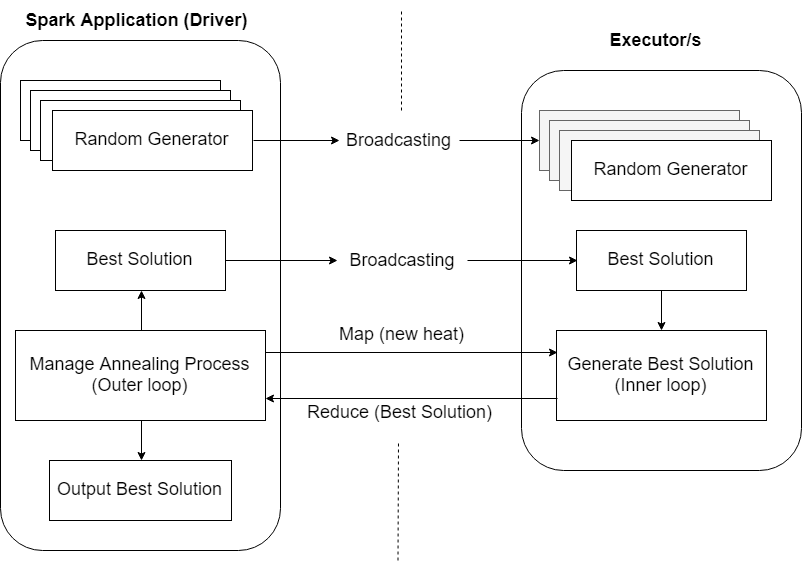
\includegraphics[scale=0.45]{spark_flow_diagram.png}
		\end{figure}
		
		\subsection{MASS} \label{D_MASS}
			Our MASS implementation spread out computation over multiple nodes by running SA on each place individually. \\
			
			Each place received a different random seed, to ensure they did not follow the same path, and a different starting point. At the conclusion of each outer-loop iteration, all places outputs their current best solution, and all places then adopted the best solution from the list of current best solution of each place. This was done to prevent having places follow a dead-end path and keep all places searching an area of the search space known to contain good solutions. This can also lead to premature convergence, however, this was the only feasible option we could think of that did not destroy the performance by introducing an immense amount of communication. \\
			
			Another change that was made to the sequential version is that we divided the number of inner loop iterations over the number of places, i.e. if we ran SA for 100 inner loop iterations over 4 places, each node would only run 25 iterations. This approach is feasible as long as the number of inner loop iterations is sufficiently large. MASS automatically handles the number of places assigned to each node. So we created the number of places equal to the number of nodes running at the time.

\pagebreak
	
	\section{Analysis} \label{ANALYSIS}

        \subsection{Perfromance} \label{PERF}
            
            \begin{figure}[!htb] \label{F3}
				\caption{Comparison of Computation for MPI, Spark, MapReduce, and MASS}
				\centering
				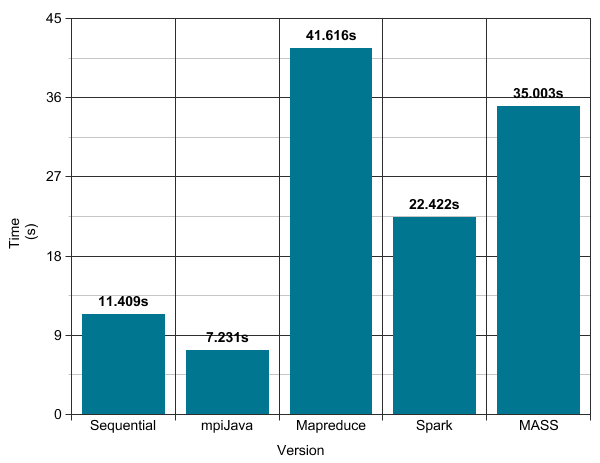
\includegraphics[scale=0.45]{performance_graph.png}
			\end{figure}
			
    		\begin{minipage}{\linewidth}
    			\centering
    			\captionof{table}{Comparison of Computation for MPI, Spark, MapReduce, and MASS} 
    			\begin{tabular}{c|cc}\label{T1}
    				Version 	& Execution Time (s)$^{\dagger}$ 	& Performance Improvement\\
    				\hline
    				Sequential	& 11.409							& N/A	\\
    				MPI Java	&  7.231							& 1.578	\\
    				MapReduce	& 41.616							& 0.274	\\
    				Spark		& 41.378							& 0.276	\\
    				MASS		& 35.003							& 0.326	\\
    				\noalign{\smallskip}\hline\noalign{\smallskip}
    				\multicolumn{3}{l}{\tiny $^\dagger$ Time of the best performing configuration of the given SA version.}
    			\end{tabular}
    			\smallskip\smallskip\smallskip\smallskip
    		\end{minipage}
        
            \subsubsection{MPI JAVA} \label{PER_MPI}
        		\begin{minipage}{\linewidth}
        			\centering
        			\captionof{table}{Comparison of Computation for MPI} 
        			\begin{tabular}{c|cc}\label{T2}
        				\# Nodes & Average Execution Time (s)$^{\dagger}$ 	& Performance Improvement	\\
        				\hline
        				1		& 32.8419									& N/A	\\
        				2		& 16.0231									& 2.050	\\
        				4		&  7.2312									& 4.542	\\
        			\noalign{\smallskip}\hline\noalign{\smallskip}
        			\multicolumn{3}{l}{\tiny $^\dagger$ Average over 100 trials}
        			\end{tabular}
        		\smallskip\smallskip\smallskip\smallskip
        		\end{minipage}
            
            \subsubsection{MapReduce} \label{PER_MR}
        		\begin{minipage}{\linewidth}
                    \centering
        			\captionof{table}{Comparison of Computation for MapReduce} 
        			\begin{tabular}{c|cc}\label{T3}
        				\# Nodes & Average Execution Time (s) & Performance Improvement\\
        				\hline
        				1	& 55.972	& N/A\\
        				2	& 41.616	& 1.345\\
        				4	& 44.423	& 1.256\\
        			\noalign{\smallskip}\hline\noalign{\smallskip}
        			\end{tabular}
        		\smallskip\smallskip\smallskip\smallskip
                \end{minipage}
                
                MapReduce is designed to work efficiently with Big Data. In our algorithm the input data is tiny. The main focus is the iterative computation of intermediate solution. Such algorithms are not not the best choice to be implemented in MapReduce. Which results in the performance to be significantly lower than the sequential version. One way the performance could be improved is by making the number of cities in the input file very large. This would definitely show better performance than the sequential version.
            
            \subsubsection{Spark} \label{PER_SPARK}
        		\begin{minipage}{\linewidth}
        			\centering
        			\captionof{table}{Comparison of Computation for Spark} 
        			\begin{tabular}{c|cc}\label{T4}
        				\# Nodes  	& Average Execution Time (s) 	& Performance Improvement	\\
        				\hline
        				1			& 36.866			& N/A	\\
        				2			& 23.620			& 1.56	\\
        				4			& 22.422 			& 1.644	\\
        			\end{tabular}
        		\smallskip\smallskip\smallskip\smallskip
				\end{minipage}

				In Spark, the user cannot assign a specific task to a designated node. On other words, the number of tasks and in which node they will be executed is managed implicitly by the driver program using DAG-Scheduler and Task Scheduler. Thus, the number of partitions used to ensure there will be at least the same number of tasks to utilize all node in the cluster. The number of partitions is changed based on the number of server nodes.
    		
    		\subsubsection{MASS} \label{PER_MASS}
        		\begin{minipage}{\linewidth}
                    \centering
        			\captionof{table}{Comparison of Computation for MASS} 
        			\begin{tabular}{c|cc}\label{T5}
        				\# Nodes & Average Execution Time (s) & Performance Improvement\\
        				\hline
        				1	& 35.003	& N/A\\
        				2	& 41.684	& 0.839\\
        				4	& 58.490	& 0.598\\
        			\noalign{\smallskip}\hline\noalign{\smallskip}
        			\end{tabular}
        		\smallskip\smallskip\smallskip\smallskip
                \end{minipage}
		
		\subsection{Programability} \label{PROG}


\pagebreak
	
	\section{Source Code} \label{SRC}
		\subsection{Program 5} \label{P5_SRC}
		The source codes for Program 5 can be found in the included src folder.\\
	
	
		\subsection{Laboratory 5} \label{L5_SRC}
			The source code for laboratory 5 is shown below and is also in the included src folder.\\
			For our laboratory, we modified the Matrix, Nomad, and QuickStart classes to build a 2D Places of size 10 x 10, populated with 10 Agents that moved through the Places migrate according to the function: $x_{new} = x_{old} * 8 + 2$ and $y_{new} = y_{old} * 2 - 4$.
			\begin{lstlisting}
			\* Agent Class *\
public class AgentX extends Agent {

	public static final int GET_HOSTNAME = 0;
	public static final int MIGRATE = 1;
	
	
	/**
	* This constructor will be called upon instantiation by MASS
	* The Object supplied MAY be the same object supplied when Places was created
	* @param obj
	*/
	public AgentX(Object obj) { }
	
	/**
	* This method is called when "callAll" is invoked from the master node
	*/
	public Object callMethod(int method, Object o) {
		switch (method) {
			case GET_HOSTNAME:
				return findHostName(o);
			case MIGRATE:
				return move(o);		
			default:
				return new String("Unknown Method Number: " + method);
		}
	}
	
	/**
	* Return a String identifying where this Agent is actually located
	* @param o
	* @return The hostname (as a String) where this Agent is located
	*/
	public Object findHostName(Object o){
		try{
			return (String) "Agent located at: " + InetAddress.getLocalHost().getCanonicalHostName() + " " + Integer.toString(getIndex()[0]) + ":" + Integer.toString(getIndex()[1]) + ":" + Integer.toString(getIndex()[2]);
		}catch(Exception e) {
			return "Error : " + e.getLocalizedMessage() + e.getStackTrace();
		}    
	}
	
	/**
	* Move this Agent to the next position in the X-coordinate
	* @param o
	* @return
	*/
	public Object move(Object o) {
	
		int xModifier = this.getPlace().getIndex()[0] * 8 + 2;
		int yModifier = this.getPlace().getIndex()[1] * 2 - 4;	        
		
		migrate(xModifier, yModifier);
		return o;
	}
}
			
			
			\* Places Class *\
			
public class Coords extends Place {
	public static final int GET_HOSTNAME = 0;
	
	/**
	* This constructor will be called upon instantiation by MASS
	* The Object supplied MAY be the same object supplied when Places was created
	* @param obj
	*/
	public Coords(Object obj) { }
	
	/**
	* This method is called when "callAll" is invoked from the master node
	*/
	public Object callMethod(int method, Object o) {
		switch (method) {
		case GET_HOSTNAME:
			return findHostName(o);
		default:
			return new String("Unknown Method Number: " + method);
		}
	}
	
	/**
	* Return a String identifying where this Place is actually located
	* @param o
	* @return The hostname (as a String) where this Place is located
	*/
	public Object findHostName(Object o){
	
		try{
			return (String) "Place located at: " + InetAddress.getLocalHost().getCanonicalHostName() +" " + Integer.toString(getIndex()[0]) + ":" + Integer.toString(getIndex()[1]) + ":" + Integer.toString(getIndex()[2]);
		}catch (Exception e) {
			return "Error : " + e.getLocalizedMessage() + e.getStackTrace();
		}
	}
}		


			\* Main Class *\
			
public class Main {
	private static final String NODE_FILE = "nodes.xml";	
 
	public static void main( String[] args ) {
		// remember starting time
		long startTime = new Date().getTime();
		
		// init MASS library
		MASS.setNodeFilePath( NODE_FILE );
		MASS.setLoggingLevel( LogLevel.DEBUG );
		
		// start MASS
		MASS.init();
		
		int x = 10;
		int y = 10;

		// initialize a 2D places object
		Places places = new Places( 1, Coords.class.getName(), ( Object ) new Integer( 0 ), x, y );
		
		// initialize some Agents
		Agents agents = new Agents( 1, AgentX.class.getName(), null, places, x);

		// instruct agents to move once
		agents.callAll(AgentX.MIGRATE);
		agents.manageAll();

		// stop MASS
		MASS.finish();
		
		// calculate / display execution time
		long execTime = new Date().getTime() - startTime;
		System.out.println( "Execution time = " + execTime + " milliseconds" );
	}
}
			
			
			\end{lstlisting}
			
	
	\section{Output} \label{OUT}
	
		\subsection{Program 5} \label{P5_OUT}		
			\begin{lstlisting}
/** Sequential Program **/
java SA 1000000 ../input_files/cities.txt
Best solution found:path: 21 -> 27 -> 24 -> 25 -> 7 -> 31 -> 2 -> 22 -> 18 -> 12 -> 15 -> 28 -> 26 -> 4 -> 20 -> 9 -> 32 -> 14 -> 8 -> 34 -> 30 -> 19 -> 13 -> 23 -> 6 -> 10 -> 35 -> 5 -> 0 -> 11 -> 33 -> 17 -> 29 -> 3 -> 1 -> 16 | distance: 447.38786463942176
Elapsed time:11409 ms.

--------------------------------------------

/** MPI Program **/
run_mpi 4 Runner 2000000 ../input_files/cities.txt
Solution is:path: 21 -> 27 -> 24 -> 25 -> 7 -> 31 -> 2 -> 22 -> 18 -> 12 -> 15 -> 28 -> 26 -> 4 -> 20 -> 9 -> 32 -> 14 -> 8 -> 34 -> 30 -> 19 -> 13 -> 23 -> 6 -> 10 -> 35 -> 5 -> 0 -> 11 -> 33 -> 17 -> 29 -> 3 -> 1 -> 16 | distance: 447.38786463942176
Execution time: 7898 ms.

-------------------------------------------

/** MapReduce Program **/
hadoop jar TspRunner.jar TspRunner 1000000 input output
18/12/10 13:27:14 WARN mapred.JobClient: Use GenericOptionsParser for parsing the arguments. Applications should implement Tool for the same.
18/12/10 13:27:14 INFO mapred.FileInputFormat: Total input paths to process : 1
18/12/10 13:27:14 INFO mapred.JobClient: Running job: job_201812101217_0007
18/12/10 13:27:15 INFO mapred.JobClient:  map 0% reduce 0%
18/12/10 13:27:39 INFO mapred.JobClient:  map 75% reduce 0%
18/12/10 13:27:45 INFO mapred.JobClient:  map 100% reduce 0%
18/12/10 13:27:48 INFO mapred.JobClient:  map 100% reduce 16%
18/12/10 13:27:54 INFO mapred.JobClient:  map 100% reduce 100%
18/12/10 13:27:56 INFO mapred.JobClient: Job complete: job_201812101217_0007
18/12/10 13:27:56 INFO mapred.JobClient: Counters: 19
18/12/10 13:27:56 INFO mapred.JobClient:   Map-Reduce Framework
18/12/10 13:27:56 INFO mapred.JobClient:     Combine output records=4
18/12/10 13:27:56 INFO mapred.JobClient:     Spilled Records=8
18/12/10 13:27:56 INFO mapred.JobClient:     Reduce input records=4
18/12/10 13:27:56 INFO mapred.JobClient:     Reduce output records=1
18/12/10 13:27:56 INFO mapred.JobClient:     Map input records=4
18/12/10 13:27:56 INFO mapred.JobClient:     Map output records=4
18/12/10 13:27:56 INFO mapred.JobClient:     Map output bytes=972
18/12/10 13:27:56 INFO mapred.JobClient:     Reduce shuffle bytes=813
18/12/10 13:27:56 INFO mapred.JobClient:     Combine input records=4
18/12/10 13:27:56 INFO mapred.JobClient:     Map input bytes=814
18/12/10 13:27:56 INFO mapred.JobClient:     Reduce input groups=1
18/12/10 13:27:56 INFO mapred.JobClient:   FileSystemCounters
18/12/10 13:27:56 INFO mapred.JobClient:     HDFS_BYTES_READ=2041
18/12/10 13:27:56 INFO mapred.JobClient:     FILE_BYTES_WRITTEN=2278
18/12/10 13:27:56 INFO mapred.JobClient:     FILE_BYTES_READ=1066
18/12/10 13:27:56 INFO mapred.JobClient:     HDFS_BYTES_WRITTEN=261
18/12/10 13:27:56 INFO mapred.JobClient:   Job Counters
18/12/10 13:27:56 INFO mapred.JobClient:     Launched map tasks=4
18/12/10 13:27:56 INFO mapred.JobClient:     Launched reduce tasks=1
18/12/10 13:27:56 INFO mapred.JobClient:     Rack-local map tasks=1
18/12/10 13:27:56 INFO mapred.JobClient:     Data-local map tasks=3
Execution Time: 42553ms

hadoop fs -cat /user/anjald_css534/output/part-00000
Best Solution Found:    path: 21 -> 27 -> 24 -> 25 -> 7 -> 31 -> 2 -> 22 -> 18 -> 12 -> 15 -> 28 -> 26 -> 4 -> 20 -> 9 -> 32 -> 14 -> 8 -> 34 -> 30 -> 19 -> 13 -> 23 -> 6 -> 10 -> 35 -> 5 -> 0 -> 11 -> 33 -> 17 -> 29 -> 3 -> 1 -> 16 | distance: 447.38786463942176

--------------------------------------------

/** Spark Program **/
spark-submit --class uwb.css534.prog5.App --master "spark://cssmpi1.uwb.edu:60007" --total-executor-cores 12 sa-tsp-spark-1.0-SNAPSHOT.jar 2000000 CSS534_Program5/code/input_files/cities.txt 12
Best solution found:path: 21 -> 27 -> 24 -> 25 -> 7 -> 31 -> 2 -> 22 -> 18 -> 12 -> 15 -> 28 -> 26 -> 4 -> 20 -> 9 -> 32 -> 14 -> 8 -> 34 -> 30 -> 19 -> 13 -> 23 -> 6 -> 10 -> 35 -> 5 -> 0 -> 11 -> 33 -> 17 -> 29 -> 3 -> 1 -> 16 | distance: 447.38786463942176
Elapsed time:15438 ms.

spark-submit --class uwb.css534.prog5.App --master "spark://cssmpi1.uwb.edu:60007" --total-executor-cores 12 sa-tsp-spark-1.0-SNAPSHOT.jar 10000000 CSS534_Program5/code/input_files/cities.txt 100
Best solution found:path: 21 -> 27 -> 24 -> 25 -> 7 -> 31 -> 2 -> 22 -> 18 -> 12 -> 15 -> 28 -> 26 -> 4 -> 20 -> 9 -> 32 -> 14 -> 8 -> 34 -> 30 -> 19 -> 13 -> 23 -> 6 -> 10 -> 35 -> 5 -> 0 -> 11 -> 33 -> 17 -> 29 -> 3 -> 1 -> 16 | distance: 447.38786463942176
Elapsed time:29135 ms.
--------------------------------------------

/** MASS Program **/
java -jar prog5-1.0-SNAPSHOT.jar 2000000 cities.txt 4
MProcess on v0243p.host.s.uw.edu run with command: java -Xmx9g -cp /home/anjald_css534/prog5/.jar edu.uw.bothell.css.dsl.MASS.MProcess v0243p.host.s.uw.edu 1 4 1 58136 /home/anjald_css534/prog5
MProcess on v0244p.host.s.uw.edu run with command: java -Xmx9g -cp /home/anjald_css534/prog5/.jar edu.uw.bothell.css.dsl.MASS.MProcess v0244p.host.s.uw.edu 2 4 1 58136 /home/anjald_css534/prog5
MProcess on v0245p.host.s.uw.edu run with command: java -Xmx9g -cp /home/anjald_css534/prog5/.jar edu.uw.bothell.css.dsl.MASS.MProcess v0245p.host.s.uw.edu 3 4 1 58136 /home/anjald_css534/prog5
MASS.init: done
Best Solution:path: 21 -> 27 -> 24 -> 25 -> 7 -> 20 -> 4 -> 26 -> 28 -> 31 -> 2 -> 22 -> 18 -> 12 -> 15 -> 16 -> 1 -> 3 -> 29 -> 17 -> 33 -> 11 -> 0 -> 5 -> 35 -> 10 -> 6 -> 23 -> 13 -> 19 -> 30 -> 34 -> 8 -> 14 -> 32 -> 9 | distance: 449.6584675618958
Execution time = 57156 milliseconds


			\end{lstlisting}	
	
\end{document}